%; whizzy chapter
% -initex iniptex -latex platex -format platex -bibtex jbibtex -fmt fmt
% 以上 whizzytex を使用する場合の設定。

%     Tokyo Debian Meeting resources
%     Copyright (C) 2010 Junichi Uekawa

%     This program is free software; you can redistribute it and/or modify
%     it under the terms of the GNU General Public License as published by
%     the Free Software Foundation; either version 2 of the License, or
%     (at your option) any later version.

%     This program is distributed in the hope that it will be useful,
%     but WITHOUT ANY WARRANTY; without even the implied warranty of
%     MERCHANTABILITY or FITNESS FOR A PARTICULAR PURPOSE.  See the
%     GNU General Public License for more details.

%     You should have received a copy of the GNU General Public License
%     along with this program; if not, write to the Free Software
%     Foundation, Inc., 51 Franklin St, Fifth Floor, Boston, MA  02110-1301 USA

%  preview (shell-command (concat "evince " (replace-regexp-in-string "tex$" "pdf"(buffer-file-name)) "&"))
% 画像ファイルを処理するためにはebbを利用してboundingboxを作成。
%(shell-command "cd image201007; ebb *.jpg")

%%ここからヘッダ開始。

\documentclass[mingoth,a4paper]{jsarticle}
\usepackage{monthlyreport}

% 日付を定義する、毎月変わります。
\newcommand{\debmtgyear}{2010}
\newcommand{\debmtgmonth}{7}
\newcommand{\debmtgdate}{17}
% (+ (* (- 2010 2005) 12) 6) started from zero
\newcommand{\debmtgnumber}{66} 

\begin{document}


\begin{titlepage}
\thispagestyle{empty}
% タイトルページ:編集必要な部分は最初のマクロに飛ばすこと

\vspace*{-2cm}
第\debmtgnumber{}回 東京エリア Debian 勉強会資料\\
\hspace*{-2cm}

\includegraphics[width=210mm]{image201003/debsen.eps}\\
\hfill{}\debmtgyear{}年\debmtgmonth{}月\debmtgdate{}日

% ここはアップデートすること
\rotatebox{10}{\fontsize{32}{32} {\gt 特集1: 俺のDebianな一日}}

\rotatebox{10}{\fontsize{32}{32} {\gt 特集2: libsaneとの格闘} }

\vspace*{-2cm}
\hfill{}
\includegraphics[height=6cm]{image200502/openlogo-nd.eps}
\end{titlepage}

\dancersection{Introduction}{上川 純一}

\begin{multicols}{2}
 

 今月のDebian勉強会へようこそ。これからDebianの世界にあしを踏み入れると
 いう方も、すでにどっぷりとつかっているという方も、月に一回Debianについ
 て語りませんか?

 Debian勉強会の目的は下記です。

 \begin{itemize}
 \item \underline{Debian Developer} (開発者)の育成。
 \item 日本語での「\underline{開発に関する情報}」を整理してまとめ、アップデートする。
 \item \underline{場}の提供。
 \begin{itemize}
  \item 普段ばらばらな場所にいる人々が face-to-face で出会える場を提供
	する。
  \item Debian のためになることを語る場を提供する。
  \item Debianについて語る場を提供する。
 \end{itemize}
 \end{itemize}		

 Debianの勉強会ということで究極的には参加者全員がDebian Packageをがりがり
 と作るスーパーハッカーになった姿を妄想しています。情報の共有・活用を通し
 て Debianの今後の能動的な展開への土台として、「場」としての空間を提供す
 るのが目的です。

\end{multicols}

\newpage

\begin{minipage}[b]{0.2\hsize}
 \definecolor{titleback}{gray}{0.9}
 \colorbox{titleback}{\rotatebox{90}{\fontsize{80}{80} {\gt デビアン勉強会} }}
\end{minipage}
\begin{minipage}[b]{0.8\hsize}
\hrule
\vspace{2mm}
\hrule
\begin{multicols}{2}
\tableofcontents
\end{multicols}
\vspace{2mm}
\hrule
\end{minipage}

\dancersection{事前課題}{上川 純一}

今回の事前課題は以下です:

\begin{enumerate}
 \item 俺のDebianな一日
\end{enumerate}

この課題に対して提出いただいた内容は以下です。

% 
\begin{prework}{ $BOBED7r(B }

$BIaCJ;H$C$F$$$k(BLinux$B%G%#%9%H%j%S%e!<%7%g%s!'(BDebian /GNU Linux
$B;H$C$F$_$?$$(BLinux$B%G%#%9%H%j%S%e!<%7%g%s!'FC$K$J$7(B
$B;H$C$F$$$kM}M3!'%Q%C%1!<%84IM}$,3Z(B
$BL%NO!'%Q%C%1!<%84IM}$,3Z(B
$BITK~!'FC$K$J$7(B


\end{prework}



\begin{prework}{ $BF#BtM}Ao(B(risou) }

$BIaCJ;H$C$F$$$k%G%#%9%H%j%S%e!<%7%g%s$O(BDebian$B$H(BRedHat$B!#(B
RedHat$B$O;E;v$G$7$+;H$C$F$^$;$s!#(BDebian$B$r;H$C$F$kM}M3$OBg3X;~Be$K=jB0$7$F$$$?8&5f<<$N%5!<%P$,(BDebian$B$@$C$?$+$i!#B>$N%G%#%9%H%j%S%e!<%7%g%s$K?($l$k5!2q$b$"$C$?$1$l$I!"7k6I0lHV;H$$$J$l$?$b$N$r$:$C$H;H$C$F$$$k46$8$G$9!#;H$C$F$_$?$$%G%#%9%H%j%S%e!<%7%g%s$O!"(BUbuntu$B$d(BGentoo$B$J$I!#:#$^$G;H$&5!2q$,$J$+$C$?$N$G!"0lEY;H$C$F$_$?$$!"$H$$$&4JC1$JF05!$G$9!#(B

\end{prework}



\begin{prework}{ $B5HLn(B(yy\_y\_ja\_jp) }

$BIaCJ(B Debian $B$r;H$C$F$$$^$9!%?'!9$J0UL#$G<+M3$@$+$i$G$9!%ITK~$O$"$^$j46$8$F$^$;$s!%(BUbuntu $B$5$s$O$h$j(B global $B$J(B Debian $B$K$b$C$H@.2L$r4T85$7$F$$$?$@$1$k$H$&$l$7$/;W$$$^$9!%(B

\end{prework}



\begin{prework}{ $B868}=(9/(B }

debian
$B7Z$$(B

$B8D?ME*$K$O(Bubuntu$B$G$9$,(B
$B2q<R$,(Bred hat$B$r;HMQ$7$F$$$k$N$G(Bred hat$B$K$b6=L#$,$"$j$^$9!#(B

\end{prework}



\begin{prework}{ hard2259 }

$BIaCJ;H$C$F$$$k(BLinux$B%G%#%9%H%j%S%e!<%7%g%s(B
\begin{itemize}
\item VineLinux
\item Ubuntu
\item CentOS
\end{itemize}

$B;H$C$F$$$kM}M3(B

\begin{itemize}
\item Vine\\
$B!!"13X9;$N<x6H$G;XDj$5$l$F$k$+$i!#(B\\
  $B"1$$$$0UL#$G8O$l$?5;=Q$H$$$o$l$?$b$N$rB?$/;H$C$F$$$k$?$a!"(BLinux$B7O$r0l$+$iJY6/$9$k$K$O$b$C$F$3$$$N%b%N$i$7$$$N$G!#(B\\

\item Ubuntu \\
$B!!"1%<%_<<$N@hGZ$+$i4+$a$i$l$?(B
$B!!"1(BWindows$B$K6a$$%b%N$,$"$k$+$i(B

\item CentOS \\
$B!!"1%<%_<<$N%5!<%P$N(BOS$B$,(BCentOS$B$@$+$i;H$o$6$k$rF@$J$$!#(BRedHat$B7O$N9=B$$H;w$F$$$k$+$i!"2q<R$O$$$C$?$H$-LrN)$D$+$b!#(B
$B"(ITK~$r8@$($k$[$I;H$$9~$s$G$^$;$s$4$a$s$J$5$$!#(B
\end{itemize}


$B;H$C$F$_$?$$(BLinux$B%G%#%9%H%j%S%e!<%7%g%s(B\\
$B!&(BGentoo

$B;H$C$F$_$?$$M}M3(B\\
$B!&(BGentoo\\
$B!!"1?'!9Fq$7$$$H$$$o$l$F$$$k$+$iD)@o$7$F$_$?$$!#(B

\end{prework}



\begin{prework}{ $B%-%?%O%i(B }

$BIaCJ;H$C$F$$$k(BLinux$B%G%#%9%H%j%S%e!<%7%g%s(B:debian, Ubuntu
$B!!!!L5NA$G;H$($k!"%i%$%;%s%94IM}$GG:$^$J$/$FNI$$!"2?$+;H$$$?$$%=%U%H$,(B
$B$"$k$H!V(Bapt-get$B!W$G$9$0;n$;$k!#!!$G$b!"4D6-$K$h$C$F2;$,=P$J$+$C$?$j!"(B
$B%0%i%U%#%C%/$d%W%j%s%?$N%I%i%$%P$GG:$s$@$j!"(BWindows$B0MB8$N(BWeb$B%Z!<%8$K(B
$B%"%/%;%9$G$-$J$+$C$?$j!"?M$K4+$a$k$K$O>/!9G:$^$7$$=j$,$"$k!#(B

$B;H$C$F$_$?$$(BLinux$B%G%#%9%H%j%S%e!<%7%g%s(B:Ubuntu(ARM), Android(?)
$B!!!!%b%P%$%kMQES$GMxMQ$7$F$$$k!V(BZaurus$B!W$N@=IJ<wL?$,$D$-$F$$$k$N$G!"(B
$B$=$N8e7Q$H$7$F!V(BNetWalker$B!W$+!V(BJN-DK01$B!W$H$+!V(BIS01$B!W$N(BAndroid$B5!$,(B
$BM_$7$$$J$!!<$H!";W$C$F$^$7$F!&!&!&!#(B


\end{prework}



\begin{prework}{ KIM\_TPDN }

$B%G%9%/%H%C%WMQES$G(BopenSUSE$B!"(BVPS$B$G(BCentOS$B$r;H$C$F$$$^$9!#$A$J$_$K<+Bp;*$O(BFreeBSD$B$r;HMQ$7$F$$$^$9!#(B

$B;H$C$F$$$kM}M3(B
openSUSE
$B!&(BYaST$B$,$+$J$jJXMx!#(B
$B!&(BKDE$B$,9%$-!#(B

CentOS
$B!&=i$a$F;H$C$?%G%#%9%H%m$@$+$i!#0lDL$j$N$3$H$r$3$l$G3X=,$7$?!#(B
$B!&(BVPS$B$d@l;*$N(BOS$BA*Br;h$K$O$?$$$F$$F~$C$F$k!#(B

$B;H$C$F$_$?$$%G%#%9%H%j%S%e!<%7%g%s(B
$B!&(BArudius
$B!&(BUbuntu Studio



\end{prework}



\begin{prework}{ $B>e@n=c0l(B }

$B$$$^$U$H?6$jJV$k$HIaCJ$b$C$H$b;H$C$F$$$k(B Linux $B%G%#%9%H%j%S%e!<%7%g%s$O(B Android $B$G$9!#(B
$B7HBSEEOC$K%W%j%$%s%9%H!<%k$5$l$F$$$k$N$G;H$$E]$7$F$$$^$9!#(B
$BITK~E@$O%+!<%M%k$r$$$8$l$J$$$3$H$H!"(Bemacs$B$,F0$+$J$$$3$H$G$9!#(B


\end{prework}



\begin{prework}{ compozz }

$B!&IaCJ;H$C$F$$$k%G%#%9%H%j%S%e!<%7%g%s(B
$B!!(BUbuntu
$B!&;H$C$F$_$?$$%G%#%9%H%j%S%e!<%7%g%s(B
$B!!(BFedora

$B!&(B(Ubuntu$B$r(B)$B;H$C$F$$$kM}M3(B
$B!!%f!<%6!<$NB?$5$d0BDj@-$,$"$k!J$H;W$C$F$$$k!K$+$i$G$9!#(B

$B!&L%NO(B
$B!!(BKNOOPIX$B$N(BLiveCD$B$r;H$*$&$H$7$?;~!"5/F0;~$+$i%G%#%9%W%l%$%I%i%$%P$G$O$^$C$?$1$l$I!"(BUbuntu$B$O@_DjJQ99$7$J$/$F$b%$%s%9%H!<%k2hLL$+$i(BGUI$B$G46F0$7$^$7$?!#(B
$B!!$H$K$+$/(BLinux$B$NCf$G$OF3F~$d1?MQ$,3Z$@$H;W$&$N$G!"IaCJ;H$$$K$H$F$bLrN)$C$F$$$^$9!#(B

$B!&ITK~E@(B
$B!!%G%#%9%H%j%S%e!<%7%g%s$NITK~$O$[$H$s$IL5$$$G$9$,!"5M$^$C$?$H$-$K(BUbuntu$B$N%P%0$@$C$?$j$7$F$,$C$+$j$7$?$3$H$,$"$j$^$9!#(B

$B!&(B(Fedora$B$r(B)$B;H$C$F$_$?$$M}M3(B
$B!!;H$C$F$_$?$3$H$,$J$$$+$i$G$9!#(B Gentoo$B$O;~4V$,$"$l$P!#(B
Debian$BJY6/2q$J$N$K$9$_$^$;$s!#!#!#(B

\end{prework}



\begin{prework}{ mnakao }

$BIaCJ;H$C$F$$$k(BLinux$B%G%#%9%H%j%S%e!<%7%g%s!'(B
$B$=$l$O(BDebian$B$G$7$g$&!*(B

$B;H$C$F$_$?$$(BLinux$B%G%#%9%H%j%S%e!<%7%g%s!'(B
openSUSE$B$r;E;v$G>/$7;H$C$F$_$?$1$I!"7k9=JXMx$=$&$J$N$G5$$K$J$C$F$^$9!#(B

$B!J(BDebian$B$r!K;H$C$F$$$kM}M3!"L%NO!'(B
apt$B$,JXMx$J$N$H!"0lEY%$%s%9%H!<%k$7$?$i!":F%$%s%9%H!<%k$9$kI,MW$,$J$$$3$H!J;d$O%X%?%l$J$N$G!"2?EY$b%/%j!<%s%$%s%9%H!<%k$7$F$^$9$,(B:p$B!K(B

$B!J(BDebian$B$N!KITK~E@!'(B
$BF~Lg<T$O$=$NJ82=$K47$l$k$N$,BgJQ$J=j!#(B

$B!J(BSuse$B$r!K;H$C$F$_$?$$M}M3!'(B
YaST$B$,$"$k$+$i!#(BLDAP$B$N@_Dj$b(BYaST$B$G=PMh$k$N$GJXMx$=$&!#(B


\end{prework}



\begin{prework}{ koedoyoshida }

$BIaCJ;H$C$F$$$k(BLinux$B%G%#%9%H%j%S%e!<%7%g%s(B
Debian,Ubuntu,Asianux,RHEL
$B;H$C$F$_$?$$(BLinux$B%G%#%9%H%j%S%e!<%7%g%s$O2?$G$9$+!)(B
Gentoo
$B;H$C$F$$$kM}M3(B
Debian:$B%Q%C%1!<%8$,B?$$!#(Bstable$B$N%P!<%8%g%s%"%C%W$,CY$$$N$G!"%5!<%P8~$1$K0BDj$7$F$$$k!#%$%s%9%H!<%k8e$N<j4V$,3]$+$i$J$$!#(B
Ubuntu:$B%Q%C%1!<%8$,B?$$!#%+!<%M%k$,?7$7$/!"(BLiveCD$B$,I8=`$J$N$G?77?5!$G3F<o%G%P%$%9$NF0:n$r3NG'$9$k$N$KJXMx!#%$%s%9%H!<%k$N<j4V$,3]$+$i$J$$!#(B
Asianux:$BHS$N<o(B
RHEL:$BNI$/$b0-$/$bI8=`$G;29M$K$J$k(B
$BL%NO!"ITK~E@!";H$C$F$_$?$$M}M3(B
Gentoo:$B%Q%C%1!<%8$NB?$5!"<j4V$,$+$+$j$=$&$J$H$3$m!"%^%K%"8~$1(B


\end{prework}



\begin{prework}{ moli3 }

$BIaCJ;H$C$F$$$k%G%#%9%H%j%S%e!<%7%g%s(B
CentOS
$BN>J}=i?4<T$K$O$J$+$J$+Fq$7$$$h$/m5$/$3$H$,$"$j$^$9!#(B
$B%5!<%P$K8~$$$F$$$k$HJ9$$$F%5!<%P$H$7$F;H$C$F$$$^$7$?!#(B
Debian
$B:G6a%5!<%P$H%G%#%9%/%H%C%W$r%5!<%P$K$7$^$7$?!#(BCentOS$B$H0c$&E@$G(B
$B8MOG$&$H$-$,$"$j$^$9!#(B
$B;H$C$F$_$?$$%G%#%9%H%j%S%e!<%7%g%s(B
gentoo
$B$h$/$o$+$i$J$$$1$IOCBj$J$N$GF~$l$F$_$?$$$G$9!#(BDebian$B$+$i(Bchroot$B$G(B
$B$d$m$&$+$H;W$C$F$^$9!#(B

\end{prework}



\begin{prework}{ $BB<ED?.?M(B }

$B;H$C$F$$$k(B: Ubuntu
+ $BH>G/$4$H$K40@.EY$N9b$$%P!<%8%g%s$,%j%j!<%9$5$l$k$H$$$&%5%$%/%k(B
+ Humanity$B%"%$%3%s%F!<%^(B
+ Mark Shuttleworth$B$N9TF0NO(B
- Mark Shuttleworth$B$N9TF0NO(B

$B;H$C$F$_$?$$(B: Debian
stable, testing, unstable$B$rJBNs$G?J$a$F$$$k$H$3$m!#(B

\end{prework}



\begin{prework}{ akedon }

$BIaCJ;H$C$F$$$k(BLinux$B%G%#%9%H%j%S%e!<%7%g%s$O(BDebian,CentOS,MIKO GNYO/Linux (Ubuntu Desktop) $B$G$9!#(B
$B;H$C$F$_$?$$(BLinux$B%G%#%9%H%j%S%e!<%7%g%s$O(BSuSE$B$G$9$M!#(B
$BA05-$N(BLinux$B$r;H$C$F$$$kM}M3$O(BDebian$B$O;H$$;O$a$?Ev;~$O05E]E*$K(Bapt$B%D!<%k$,B>$N4IM}%D!<%k(Brpm$B$h$j;H$$$d$9$+$C$?$N$G!"$=$3$+$i;H$$B3$1$F47$l$F$$$k$+$i$G$9!#(BCentOS$B$O(BXen$B$r;H$$;O$a$?;~$K0lHV<j7Z$G3N<B$KF0$$$?$+$i$G$9!#(BMIKO GNYO/Linux$B$OJI;f$,AGE($G$9$h$M!"Mn$ACe$$$F:n6H$9$k$K$O:GE,$G$9!#(B 
$BL%NO$O(BLinux$BA4BN$K8@$($k$3$H$G$9$,!"ITMW$J5!G=$r;_$a$?$j:o=|$7$?$j!"I,MW:GDc8B$K9J$j9~$_$d$9$/!";H$$$d$9$$MM$K%+%9%?%^%$%:$7$d$9$$$H$$$&E@$K$"$j$^$9!#(B
$BITK~E@$O!"%G%P%$%9%I%i%$%PEy!"%Y%s%@$K0MB8$7$F$$$k$b$N$,(BWindows$B$d(BMacOS$B$K8+Nt$j$9$k$b$N$,$"$C$?$j$9$kE@$K$J$j$^$9!#(B
SuSE$B$r;H$C$F$_$?$$M}M3$OC1=c$G!"L$$@;n$7$F$$$J$$$+$i$G$9!#(B

\end{prework}



\begin{prework}{ yama1066 }

$BIaCJ;H$C$F$$$k(BLinux$B%G%#%9%H%j%S%e!<%7%g%s!'(B
Debian GNU/Linux (sid, squeeze on lenny)
$B;H$C$F$$$kM}M3!'$J$s$H$J$/!#(B
$BL%NO!'$J$K$+$"$C$?$+$J!)!J$*(B
$BITK~E@!'FC$KL5$7!#(B

$BIaCJ;H$C$F$O$$$J$$$,!"(Bapt-get upgrade $B$@$1$7$F$$$k(BLinux$B%G%#%9%H%j%S%e!<%7%g%s!'(B
Ubuntu Linux (maverick)
$B;H$C$F$$$kM}M3!';H$C$F$J$$!#(B
$BL%NO!'(BDebian$B>e$G$b(B chroot $B$G6&B82DG=!#(B
$BITK~E@!'FC$KL5$7!#(B

$B;H$C$F$_$?$$(BLinux$B%G%#%9%H%j%S%e!<%7%g%s!'(BFedora (Rawhide)
$B;H$C$F$_$?$$M}M3!'?MCl$O=EMW$@$h$M!#(B

\end{prework}



\begin{prework}{ $B4d>>(B $B?.MN(B }

$BIaCJ;H$C$F$$$k(BLinux$B%G%#%9%H%j%S%e!<%7%g%s(B
Debian, Gentoo, buildroot, openembedded, $B%*%l%*%l(Bbusybox$B%Y!<%9%G%#%9%H%j(B

$B;H$C$F$_$?$$(BLinux$B%G%#%9%H%j%S%e!<%7%g%s(B
Arch Linux $B$H$+!#$J$s$+?M5$$,$"$k$h$&$G$9!#(B
$B;H$C$F$$$kM}M3!"L%NO!"ITK~E@!";H$C$F$_$?$$M}M3(B
Debian: $B;E;v$H3+H/MQ!#(B
Gentoo: $B3+H/MQ$G<g$K(BGCC$B$N(BHEAD$B$rDI$C$+$1$k$N$K;H$C$F$$$^$9!#(B
buildroot: $B;E;v$G!#%/%m%9%3%s%Q%$%i$H$+0l<0$r$H$j$"$($::n$k>l9g$KMxMQ$7$F$$$^$9!#%G%#%9%H%j$H$$$&$N$+$OITL@!#(B
openembedded: $B:G6a$$$8$j$O$8$a$^$7$?!#(Bsh$B%5%]!<%H$H$+!#(B
$B%*%l%*%l(Bbusybox$B%Y!<%9%G%#%9%H%j(B: 


\end{prework}



\begin{prework}{ monoqlo }

$BIaCJ;H$C$F$$$k(BLnux$B%G%#%9%H%j%S%e!<%7%g%s!'(BUbuntu
$B;H$C$F$_$?$$(BLinux$B%G%#%9%H%j%S%e!<%7%g%s!'$7$P$i$/(BUbuntu$B$G$$$$$G$9!#(B
$B;H$C$F$$$kM}M3!'F|K\8l$N>pJs$,$?$/$5$s$"$k$3$H$H!"=i$a$F(BLinux$B$r;H$*$&$H;W$C$?;~$K(BWindows$B$+$i$N0\9T$,3Z$@$H46$8$?$?$a!#(B
$BL%NO!'=i?4<T$K$b4+$a$d$9$$(B
$BITK~E@!'$H$/$K$J$7(B

\end{prework}



\begin{prework}{ $B$J$+$*$1$$$9$1(B }

$B;H$C$F$$$k%G%#%9%H%j%S%e!<%7%g%s$O(BDebian$B$G!"D94|E*$K;H$($=$&$J$N$,L%NO$G$9!#(B
$B;H$C$F$_$?$$%G%#%9%H%j%S%e!<%7%g%s$O!"(BScientific Linux$B$G$9!#(B

\end{prework}



\begin{prework}{ henrich }

$BIaCJ$O(B debian$B!"$=$N>e$N(B KVM $B$G(B fedora $B$H(B ubuntu $B$,$?$^$KF0$-$^$9!#(B

$B;H$C$F$_$?$$$N$O!D(BCentOS$B$+$J$!!#2?$,NI$$$N$+L%NO$,$h$/J,$+$i$s$N$G!#8eBg85$N(B RHEL$B!#(B2.1 $B$0$i$$$N;~$K%$%s%9%H!<%k$7$?5-21$7$+$J$$$N$G!#(B

\end{prework}



\begin{prework}{ $B$^$($@$3$&$X$$(B }

$BIaCJ;H$C$F$$$k%G%#%9%H%m$O(BDebian$B$G$9!#B>$K;H$C$F$_$?$$$N$OL5$$$G$9!#J#?t<oN`$N%"!<%-%F%/%A%c$GF1$8%7%9%F%`$r;H$($k(B($B%5%]!<%H$7$F$$$k%"!<%-%F%/%A%c$,B?$$(B)$B$N$,0lHV$NM}M3$G$9!#(B($B$$$D$b8@$C$F$$$kM}M3$HF1$8$GBe$o$j1G$($7$^$;$s$,(B)

\end{prework}



\begin{prework}{ $BAR@$8E(B $B63J?(B }

$BIaCJ(B: Fedora 11$B!#E,Ev$KF0$/$N$G!#>pJs$,B?$/$F5M$^$C$F;`$L$3$H$,>/$J$$!#JQ$K$3$@$o$j$r$b$C$F;H$C$F$k?M$,B?$$$N$G$?$^$K5DO@$,$+$_9g$o$J$/$F:$$k(B
$B;H$C$F$_$?$$(B: OpenSUSE$B!#7k9=I_5o$,9b$$$H;W$C$F$$$?$i!":G6a<~0O$G;H$C$F$$$k?M$,A}$($?$N$G!#(B

\end{prework}



\begin{prework}{ $BKYK\(B $B5.9,(B (opentaka) }

$BIaCJ;H$C$F$$$k(BLinux$B%G%#%9%H%j%S%e!<%7%g%s$H;H$C$F$_$?$$(BLinux$B%G%#%9%H%j%S%e!<%7%g%s$O2?$G$9$+!)(B
---
Gentoo Linux$B$r%a%$%s$K!"(BDebian$B$r(Beee pc$B$G;H$C$F$$$k!#(B
LFS(Linux From Scratch)$B$r;H$$$3$J$7$F$_$?$$!#(B
---

$B;H$C$F$$$kM}M3!"L%NO!"ITK~E@!";H$C$F$_$?$$M}M3$r65$($F$/$@$5$$!#(B
---
Gentoo Linux: 
Portage$B$KB?$/$N%Q%C%1!<%8$,$"$k!#(B

$BITK~E@(B: bleeding edge$B$9$.$F!"K\Ev$K(Bbleeding$B$9$k;~$,$"$k!#(B($B2u$l$k(B)
---

---
Debian(debian eee project): 
eeepc$B8~$1$N%G%#%9%H%j%S%e!<%7%g%s$G0lHV4JC1$K%$%s%9%H!<%k$G$-$=$&$@$C$?$+$i!#(B
---

\end{prework}




\dancersection{最近のDebian関連のミーティング報告}{岩松信洋}
\subsection{東京エリアDebian勉強会62回目報告}
% (query-replace-regexp "<.*?>" "")
% (query-replace-regexp "^[	 ]\+" "")

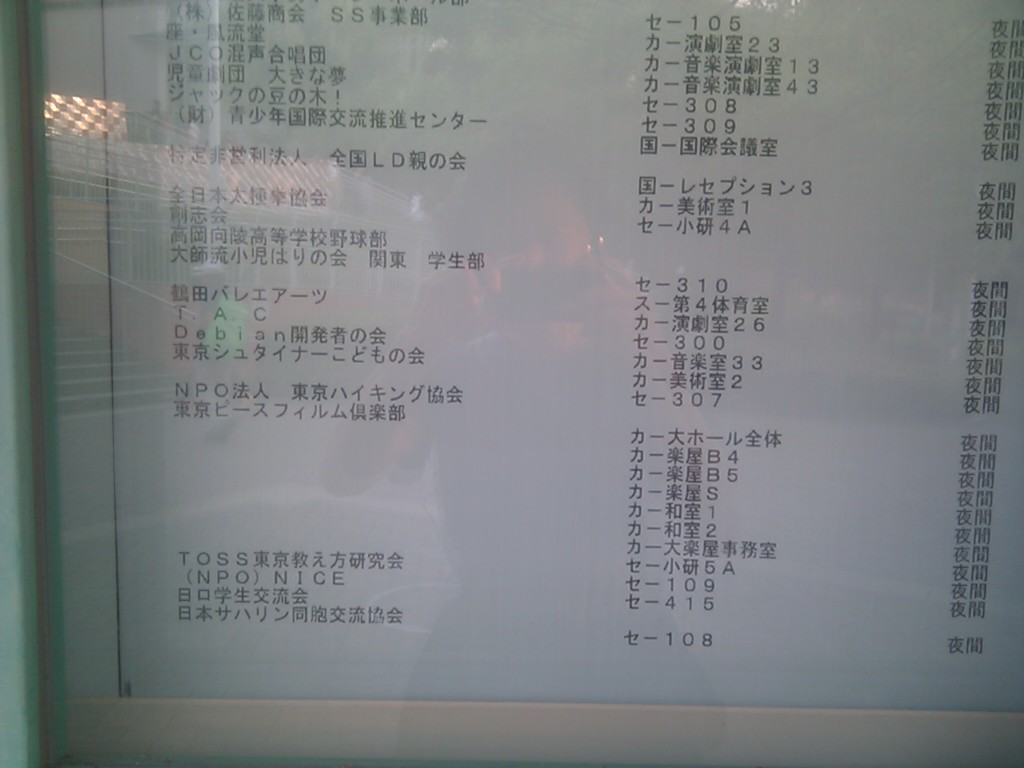
\includegraphics[width=12cm]{image201007/debianmeeting1.jpg}

今後の計画を策定しました。
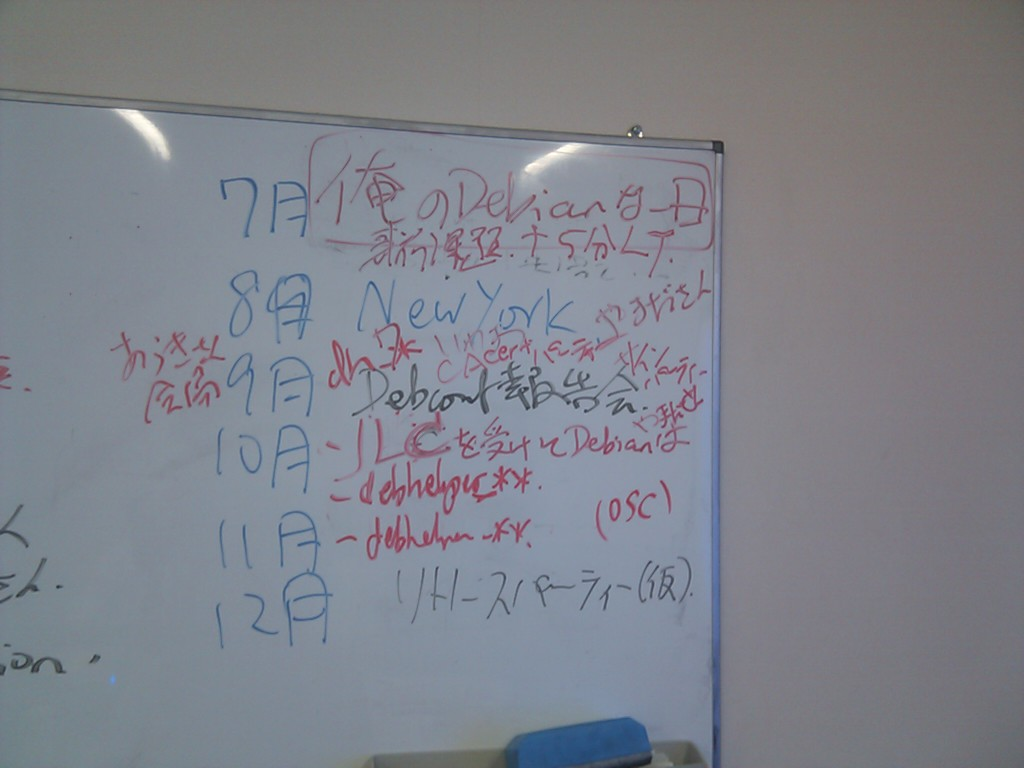
\includegraphics[width=12cm]{image201007/debianmeeting2.jpg}


\printindex

\cleartooddpage

\vspace*{15cm}
\hrule
\vspace{2mm}

\includegraphics[width=2cm]{image200502/openlogo-nd.eps}
\noindent \Large \bf Debian 勉強会資料\\ \\
\noindent \normalfont \debmtgyear{}年\debmtgmonth{}月\debmtgdate{}日 \hspace{5mm}  初版第1刷発行\\
\noindent \normalfont 東京エリア Debian 勉強会 (編集・印刷・発行)\\
\hrule

\end{document}
